\qs{Dokažte následujicí tvrzení}{
	$$ \forall n \in \mathbb{N}:  
	 1^2 + 3^2 + \ldots + (2n - 1)^2 = \frac{4n^3 - n}{3} $$
}

Výraz přepíšem do sumy.

$$ \forall n \in \mathbb{N}: \sum_{k = 1}^{n} (2k - 1)^2 = \frac{4n^3 - n}{3} $$ 

Prvně potřebujeme bázi indukce (base case). To znamená, že vložíme za $k$ jedničku.

\begin{align}
	\sum_{k = 1}^{1} (2 \cdot 1 - 1)^2 = 1
\end{align}

Náš báze je 1, je validní, báze indukce platí. Nyní provedeme indukční předpoklad a krok. Předpokládejme, že existuje nějaké $m \in \mathbb{N}$ takové, že pokud jej vložíme do $n$, tak je naše tvrzení stále platné. Pak musí platit, že i pro $m + 1$ musí naše tvrzení stále platit.

\begin{align}
	\sum_{k = 1}^{m}& (2k - 1)^2 = \frac{4m^3 - m}{3} \\
	\sum_{k = 1}^{m + 1}& (2k - 1)^2 
	= \sum_{k = 1}^{m} (2k - 1)^2 + (2(m + 1) - 1)^2
	= \frac{4(m + 1)^3 - (m + 1)}{3} \\ 
	&= \frac{4m^3 - m}{3} + (2m + 2 - 1)^2 
\end{align}

Teď, když jsme si upravili naši sumu, můžeme začít dokazovat. 

\begin{align}
	&= \frac{4m^3 - m}{3} + (2m + 2 - 1)^2 \\
	&= \frac{4m^3 - m}{3} + (2m + 1)^2 \\
	&= \frac{4m^3 - m}{3} + 4m^2 + 4m + 1 \\
	&= \frac{4m^3 - m}{3} + \frac{12m^2 + 12m + 3}{3} \\
	&= \frac{4m^3 + 12m^2 + 11m + 3}{3}
\end{align}

\begin{figure}[h]
	\centering
	\caption{Dělení polynomů $(4m^3 + 12m^2 + 11m + 3) \div (m + 1)$}
	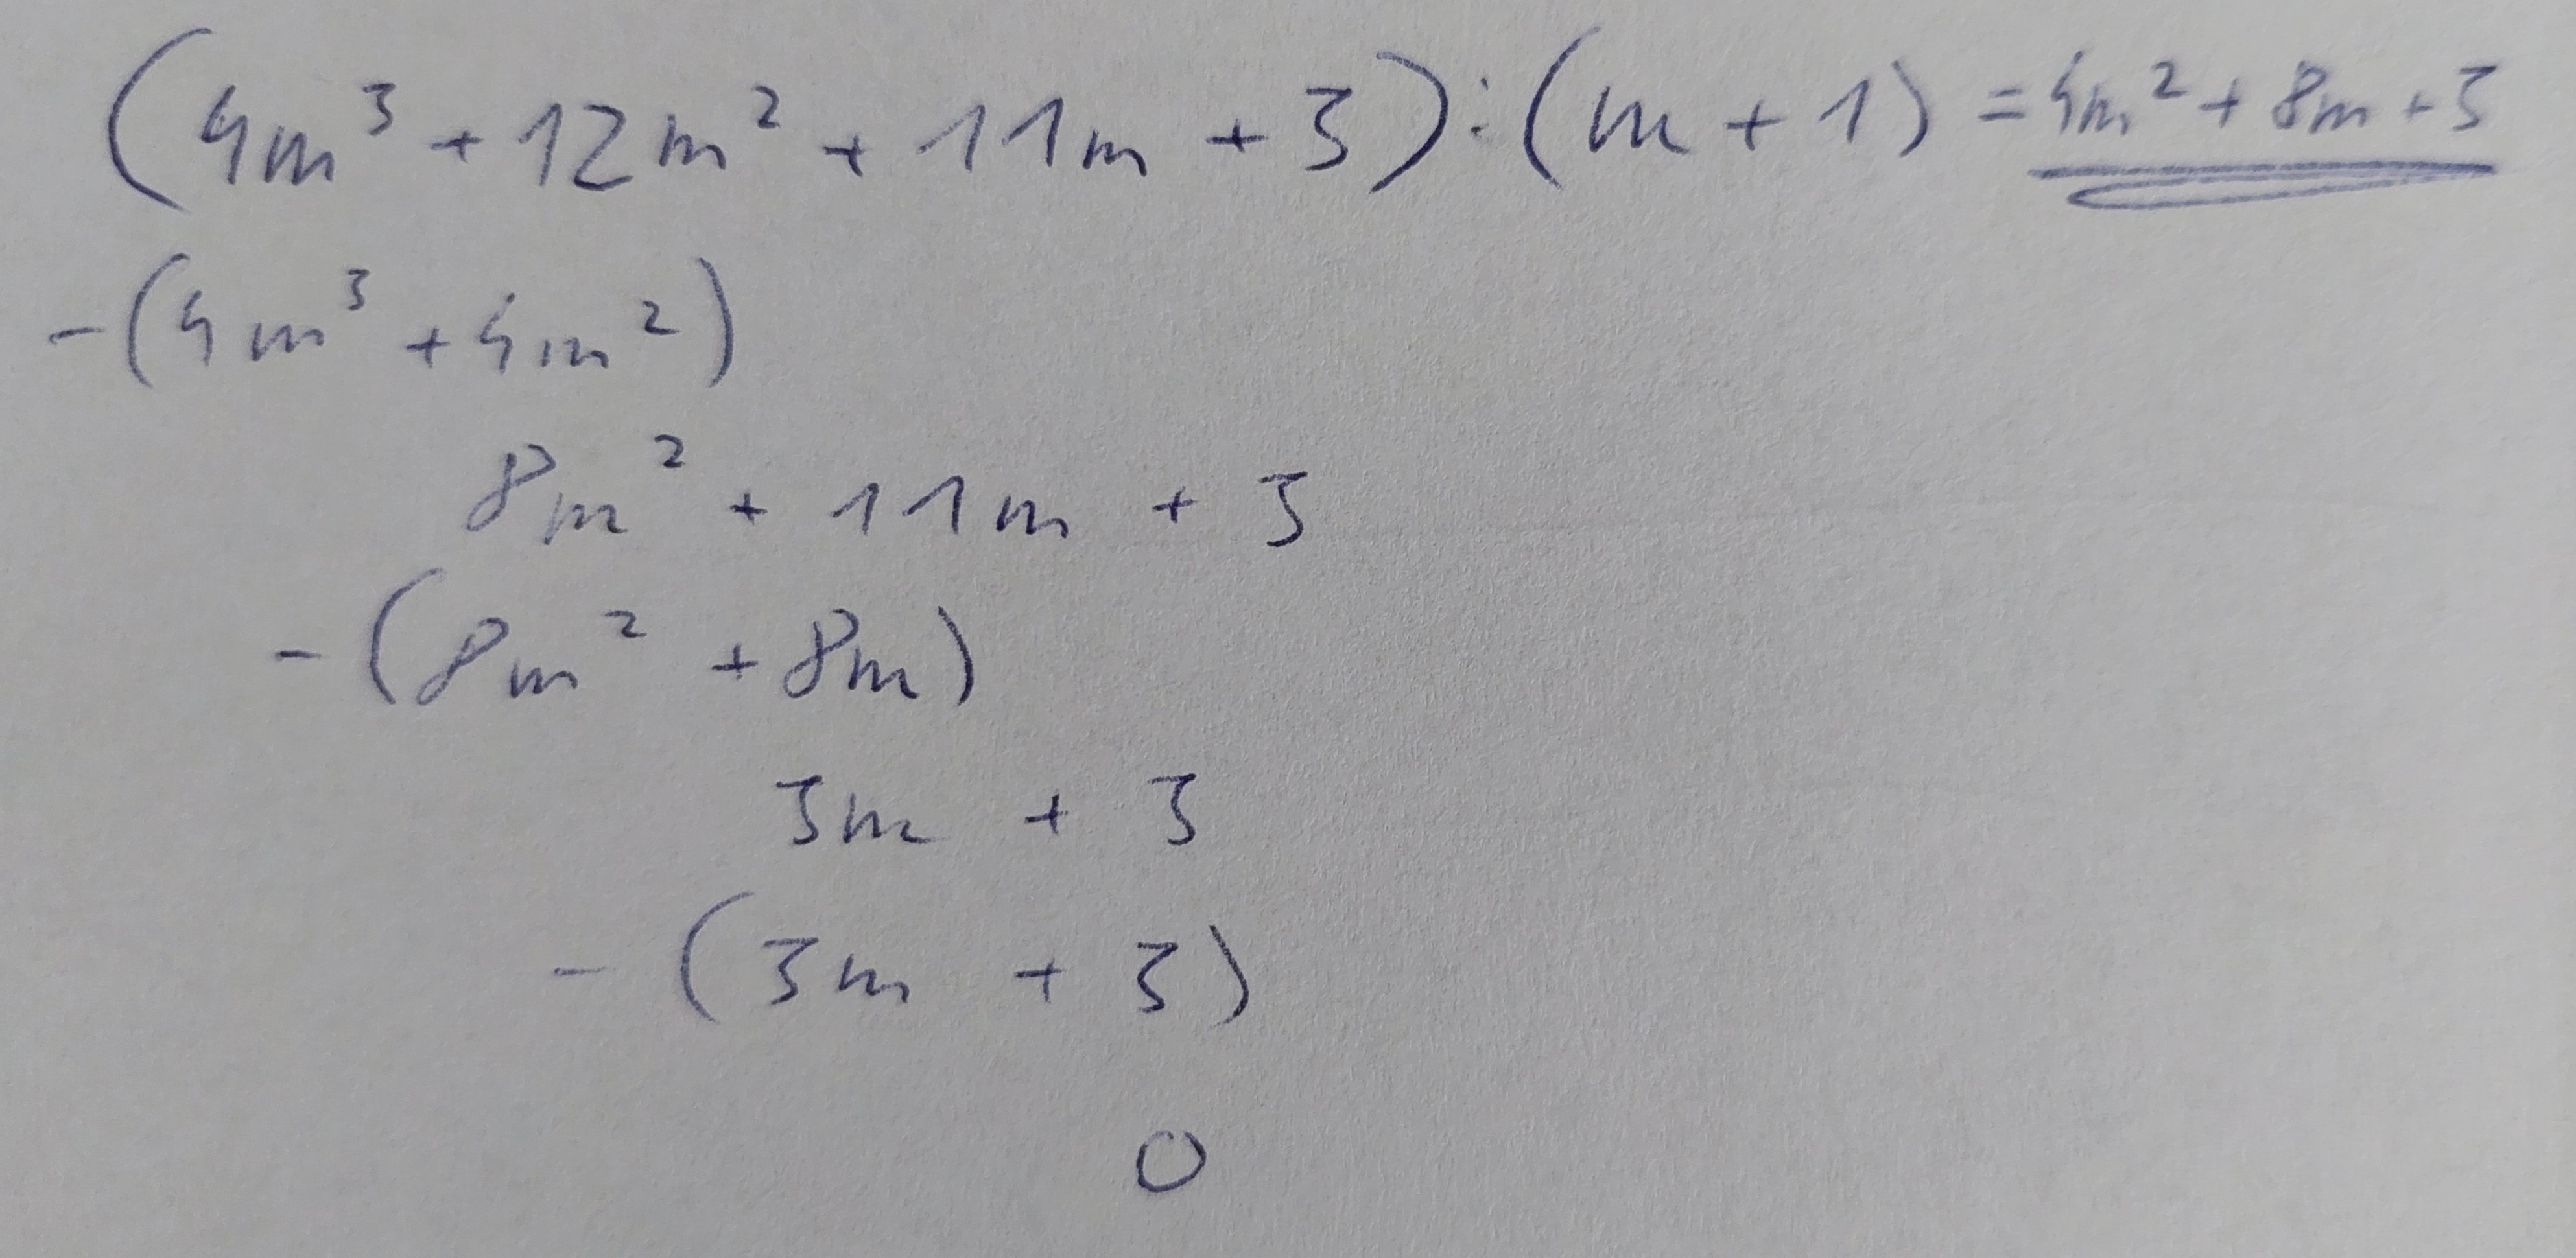
\includegraphics[width=0.8\textwidth]{assets/a1.jpg}
\end{figure}

\begin{align}
	&= \frac{(m + 1)(4m^2 + 8m + 3)}{3} \\
	&= \frac{(m + 1)(4(m^2 + 2m) + 3)}{3} \\
	&= \frac{(m + 1)(4((m^2 + 2m + 1) - 1) + 3)}{3} \\
	&= \frac{(m + 1)(4(m + 1)^2 - 4 + 3)}{3} \\
	&= \frac{(m + 1)(4(m + 1)^2 - 1)}{3} \\
	&= \frac{4(m + 1)^3 - (m + 1)}{3} 
\end{align}

Tvrzení skutečně platí.
